\begin{figure*}\centering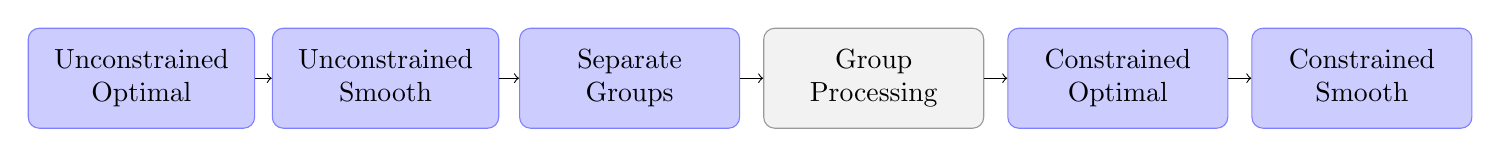
\begin{tikzpicture}
	\node[rectangle, draw=blue!50, fill=blue!20, minimum width=1.1in, minimum height=0.5in, rounded corners](problem1) at (0,0) {\begin{tabular}{c} Unconstrained \\ Optimal \end{tabular}}; 
	\node[rectangle, draw=blue!50, fill=blue!20, minimum width=1.1in, minimum height=0.5in, rounded corners](problem2) at (3.1,0) {\begin{tabular}{c} Unconstrained \\ Smooth \end{tabular}}; 
	\node[rectangle, draw=blue!50, fill=blue!20, minimum width=1.1in, minimum height=0.5in, rounded corners](problem3) at (6.2,0) {\begin{tabular}{c} Separate \\ Groups\end{tabular}}; 
	\node[rectangle, draw=gray!80, fill=gray!10, minimum width=1.1in, minimum height=0.5in, rounded corners](problem4) at (9.3,0) {\begin{tabular}{c} Group \\ Processing\end{tabular}}; 
	\node[rectangle, draw=blue!50, fill=blue!20, minimum width=1.1in, minimum height=0.5in, rounded corners](problem5) at (12.4,0) {\begin{tabular}{c}Constrained\\ Optimal \end{tabular}}; 
 	\node[rectangle, draw=blue!50, fill=blue!20, minimum width=1.1in, minimum height=0.5in, rounded corners](problem6) at (15.5,0) {\begin{tabular}{c}Constrained \\ Smooth \end{tabular}}; 
	\draw[->] (problem1.east) -- (problem2.west);
	\draw[->] (problem2.east) -- (problem3.west);
	\draw[->] (problem3.east) -- (problem4.west);
	\draw[->] (problem4.east) -- (problem5.west);
	\draw[->] (problem5.east) -- (problem6.west);
\end{tikzpicture}\caption{Overall Processing Chain}\label{fig:processChain}\end{figure*}

